% !TeX spellcheck = es_ES
\documentclass[12pt, titlepage]{article}
\usepackage[utf8]{inputenc}
\usepackage[spanish]{babel}
\usepackage{float}
\usepackage[letterpaper, margin=2.5cm]{geometry}
\usepackage[nottoc,notlot,notlof]{tocbibind} % Hace que se agregen las referencias al indice
\usepackage{url}
\usepackage{graphicx} 
\usepackage{listings}
\usepackage{color}
\definecolor{dkgreen}{rgb}{0,0.6,0}
\definecolor{gray}{rgb}{0.5,0.5,0.5}
\definecolor{mauve}{RGB}{253,151,31}

\lstset{frame=tb,
	language=Sql,
	aboveskip=3mm,
	belowskip=3mm,
	showstringspaces=false,
	columns=flexible,
	basicstyle={\small\ttfamily},
	numbers=none,
	numberstyle=\tiny\color{gray},
	keywordstyle=\color{blue},
	commentstyle=\color{dkgreen},
	stringstyle=\color{mauve},
	breaklines=true,
	breakatwhitespace=true,
	tabsize=2,
	morekeywords={use}
}

\title{Reporte: Práctica 8}
\author{Carlos Tonatihu Barrera Pérez \\ Profesor: Hernández Contreras Euler \\ Bases de Datos \\ Grupo: 2CM1 }

\begin{document}
	\maketitle
	\tableofcontents
	\section{Marco Teórico}
	Esperando que este con madre
	\section{Desarrollo}
	En esta practica se trabajan transacciones sobre la tabla tienda de la base de datos elektra, la cual ya tiene datos, las operaciones que se realizaran sobre esta tabla son similares a las que se trabajaron con la tabla cliente en el salón de clases.
	\begin{figure}[H]
		\begin{center}
			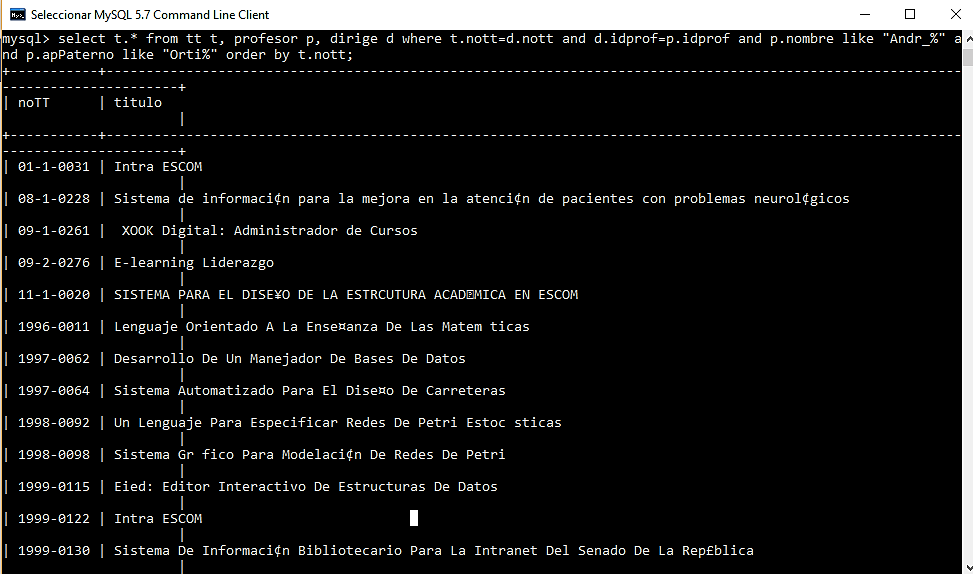
\includegraphics[width=\textwidth]{img/uno.png}
			\label{fig:uno}
			\caption{}
		\end{center}
	\end{figure}
	\begin{lstlisting}
	\end{lstlisting}

	\section{Conclusiones}
	\bibliography{bibliografia} 
	\bibliographystyle{ieeetr}
\end{document}